\begin{figure}
    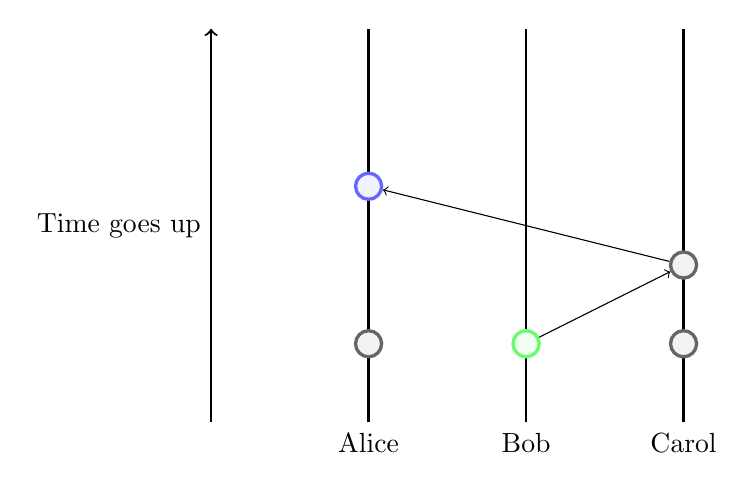
\begin{tikzpicture}[
        roundnode/.style={circle, draw=black!60, fill=black!5, very thick},
        greennode/.style={circle, draw=green!60, fill=green!5, very thick},
        bluenode/.style={circle, draw=blue!60, fill=blue!5, very thick},
        ]

        % Lines
        \draw[thick,->] (0,0) -- (0,2.5) node[anchor=east] {Time goes up} -- (0,5);
        % Alice
        \draw[thick] (2,0) node[anchor=north] {Alice} -- (2,5);
        % Bob
        \draw[thick] (4,0) node[anchor=north] {Bob} -- (4,5);
        % Carol
        \draw[thick] (6,0) node[anchor=north] {Carol} -- (6,5);

        % Nodes
        \node[roundnode] (a1) at (2,1) { };
        \node[greennode] (b1) at (4,1) { };
        \node[roundnode] (c1) at (6,1) { };
       
        % Gossips
        \node[roundnode] (c2) at (6,2) { };
        \node[bluenode] (a3) at (2,3) { };

        % Bob talks to Carol
        \draw[->] (b1) -- (c2);
        
        % Carol talks to Alice
        \draw[->] (c2) -- (a3);

    \end{tikzpicture}

    \label{fig:hashgraph}
    \caption{
        A simple example of how hashgraph spreads information via gossip.
        Bob randomly gossips to Carol, then Carol randomly gossips to Alice. Alice would have known what Bob and Carol spoke about without talking to Bob directly. This is the process of gossipping about gossip.
        Bob's green event is defined to be "strongly seen" by Alice's blue event as it was seen by at least 2/3 members along the way.
    }
\end{figure}
